\documentclass[article]{IEEEtran}
\usepackage{blindtext, graphicx, biblatex}
\addbibresource{references.bib}
\begin{document}

\title{Smart Dust Technology }
\author
{
\IEEEauthorblockN{Gerard Naughton}
\IEEEauthorblockA{Research Methods In Computing And IT\\
Software Development - Year 4\\
Galway - Mayo Institute Of Technology}
}

\maketitle

\begin{abstract}
"Smart dust" with embedded sensors, wireless communication, microprocessors and its cubic-millimeter size has revolutionized the way computers interact with the world around them. Here in my review i research the requirements, applications and hurdles facing Smart dust.
\end{abstract}


\section{Introduction}.\newline
In the fast-paced world of computing, the way we look at and perceive the computer is ever-changing. Once we reach the peak of computing power, data compaction, networking speeds or energy usage, the following day there is a another breakthrough. In the age of the Internet of Things (IoT)\cite{Lightweight}, the research community are looking for new platforms for obtaining and processing data. The introduction of Smart Dust as a platform may revolutionise this idea. 
The concept of Smart dust is the idea of  "an autonomous sensing, computing, and communication system that can be packed into a cubic-millimeter mote (a small particle or speck) to form the basis of integrated, massively distributed sensor networks"\cite{Mili}. Breakthroughs in engineering and textiles have reduced the size of these motes to cubic millimetres\cite{textiles}. Using this technology with its device size, connectivity and various sensors allows us to interact and monitor the physical world without disrupting it.\cite{MobNet}


\subsection*{History}.\newline
The idea of smart dust was first mentioned back in 1964 when Author Stanislaw Lem published the science fiction book "The Invincible". In is book he invisioned a network of tiny mechanical robots to do his will\cite{leminvincible}. It was not until 2001 that the science behind smart dust was first developed in the University of California, Berkley by professors Brett Warneke, Matt Last, Brian Liebowitz and Kristofer S.J Pister. 
Here, they developed how small computing elements and connectivity can reshape the interaction between people and computers. Their project was to explore "whether an autonomous sensing, computing, and communication system can be packed into a cubic-millimeter mote (a small particle or speck) to form the basis of integrated, massively distributed sensor networks"\cite{Mili}. 

\subsection*{What makes up a Mote?}.\newline
Here we see what components are needed to create a mote. 
Figure 1 shows a diagram of a mote. Firstly, the mote will require a power system. That is supplied by a thick film battery, a solar cell and a capacitor. Currently this technology allows us to store 1 joule per cubic millimetre. The solar cell produces 1 joule per day per square millimetre. 
The next requirement will be an integrated circuit which will process sensor data, communication, data storage and energy management. This will be the brain of the mote. 
For communication there are two method of sending and receiving data. Either through Radio Frequencies(RF) or Optical Transmission techniques. Radio Frequencies are achieved through radio wave pulses and Optical Transmission through infrared light pulses, as used in everyday devices such as remote controls. In the case of RF transmission due to limited space on a mote for a antenna and RF transmission high energy cost, Optical Transmission is the favoured choice. Transmission of data is executed in either of 2 ways; passive transmission using a corner cube retro-reflector or active transmission using a laser diode and steerable mirrors.A photodiode is used for optical data reception.
Having established the main components of the mote it is then time to choose its functionality. Here we choose which sensor technology will be attached to the mote and provide the integrated circuit raw data. Depending on the objective of the mote, various sensors may be used such as light, temperature vibration, magnetic field, acoustic and wind shear.
Finally these wireless motes will not just speak to each other but also to a main base station which can be either 10 metres away or up to a couple of kilometres.  The base station will receive data from the motes and process it into valuable information. Base stations may reside in a computer, hand held device or even in drones\cite{Mili}.

\begin{figure}[h!]
\graphicspath{ {images/} }
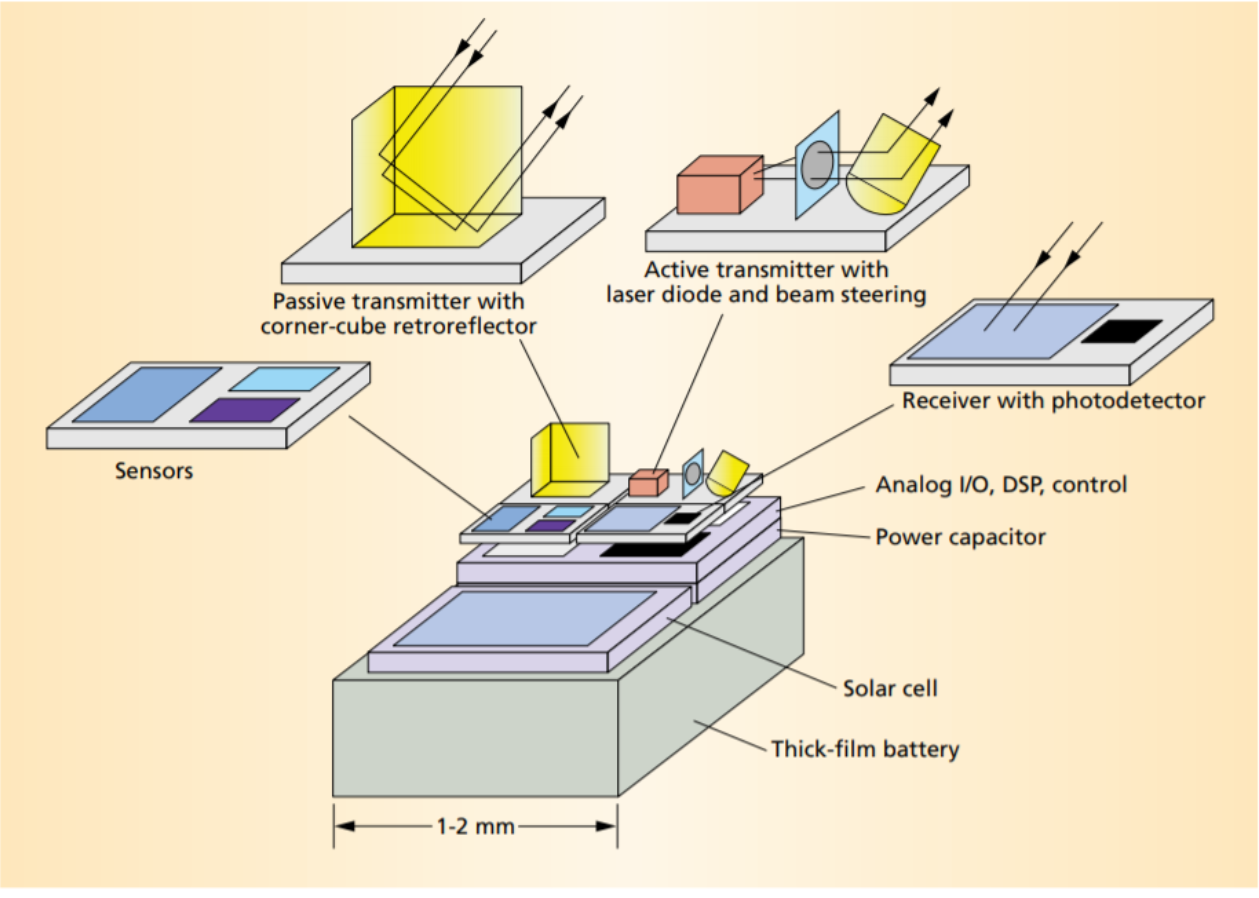
\includegraphics[width=8.8cm, height=6.5cm]{figure1}
\caption{Diagram of a Smart Dust Mote\cite{Mili}}
\end{figure}

\section{Applications}
Here we look at the applications for the technology of smart dust. It seems like the possibilities are endless but here are just some of the major ones I have found.

\subsection{Structural Health and Monitoring System}
Structural health and monitoring systems(SHM). Examples of Structural Health and Monitoring can be dated back to the beginning of the 19th Century, people known as wheel-tappers have used the sound of a hammer striking a train wheel to access if damage were present. In present day terms it was best described in the book Structural Health and Monitoring on page 6 when they defined SHM "as the use of on-structure sensing system to monitor the performance   of   the   structure   and   evaluate   its   health   state. "\cite{SHM}

Being able to detect and evaluate the safety of a structure is crucial in order to keep people safe. With aging structures and unseen damage caused to buildings, bridges and other structures through either winds, earthquakes and other extreme events. For a while now people have been implementing sensor technology into the infrastructure of buildings. Implementing wired sensors to detect the health of a structure. This comes at a cost not only for materials but also in design. A lot has to be taken into account. This also stands true for existing buildings. Trying to implement this technology into an existing structure is very hard and costly. With a lot of the key monitoring areas being inaccessible. Below in figure2 we can see the current system.

\begin{figure}[h!]
\graphicspath{ {images/} }
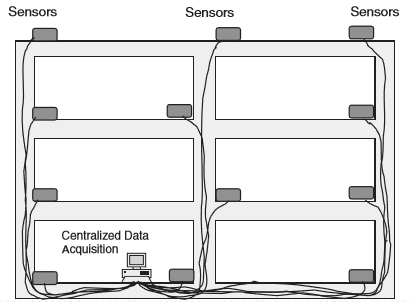
\includegraphics[width=8.8cm, height=6cm]{figure2}
\caption{Traditional SHM System adapted from \cite{SHM}}
\label{Tradition SHM}
\end{figure}

This is where Smart Dust can help. With its sensor capabilities, wireless connectivity and non-intrusive size it is perfect for the job. This will cut costs in implementation as it is wireless and only requiring millimetres of space. Also due to its tiny size the cost of smart dust is reduced also.\cite{SHM}. In figure3 we can see the smart dust sensor system.

\begin{figure}[h!]
\graphicspath{ {images/} }
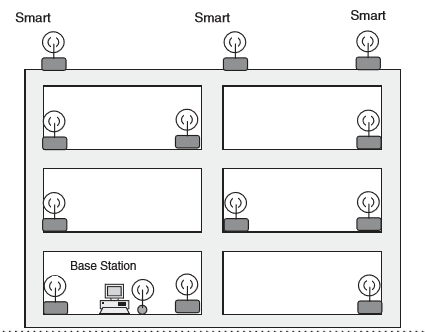
\includegraphics[width=8.8cm, height=6cm]{figure3}
\caption{Smart Sensor SHM System adapted from \cite{SHM}}
\end{figure}

\subsection{Military Applications}

As with most leading technology the Military will either have developed it or will want to use it . In this case it is no different. At the University of Berkley Kristofer S.J Pister and his group are funded by Defence Advanced research projects Agency’s(DARPA) Microsystems Technology Office\cite{Mili}. Smart Dust capabilities can be very useful to Military. Keeping troops safe is a high priority and knowing where the enemy is or whether the enemy is in your territory is essential.
Ground reconnaissance will always will be necessary but with Smart Dust this will add another dimension for keeping track of the enemy.  With Smart Dust and its cubic millimetre size it is difficult for the enemy to find or combat as the sheer amount of motes might be too great to disarm. Distribution is also made easy as it is autonomous and all self-contained. With a battery , solar cell and wireless connectivity the smart dust can be simply spread across the area in no time either by land or air\cite{Lightweight}. Using motion sensors on these motes or vibration sensors will help monitor the enemy’s movements\cite{friendorfoe}.

\subsection{Agriculture Applications}

With an ever growing world population food production is key. In many under developed countries people rely heavily on the agriculture sector to provide them food and also contribute to the countries exports. This is why monitoring of crops is essential. If a crop should fail this would lead not only less food for the people but also will affect the country’s GDP. In Hoai Bao Lam, Hiep Xuan Huynh, Pierre Yves Lucas, Mahamadou Traore and Bernard Pottier journal on monitoring environmental factors in the Mekong Delta of Vietnam. To show the importance of the Mekong Delta here are some statistics\cite{MekongDelta}

\begin{figure}[h!]
\graphicspath{ {images/} }
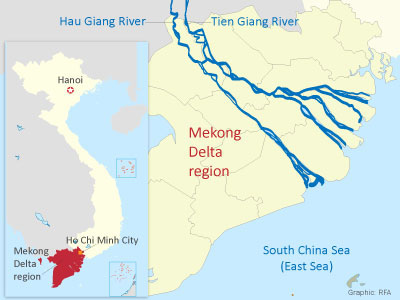
\includegraphics[width=8.8cm, height=6cm]{mekongdelta}
\caption{Map of Mekong Delta Vietnam adapted from http://www.rfa.org/english/news/vietnam/experts-warn-mekong-delta-agriculture-livelihoods-face-serious-threats-10272016103647.html/vietnam-mekong-delta-map-oct-2016-400.jpg/image}
\label{Map of Mekong Delta}
\end{figure}

The Mekong Delta is one of the most fertile plains of Southeast Asia. Stretching over 39.763 km2 and supporting a population of nearly 20 million. It is the key source of food production in Vietnam. Not only producing crops such as rice and growing fruit, the region also supports a major aquaculture. In 2012 its catfish exports reached 1.74 billion alone\cite{MekongDelta}.
Pests/insects are one such threat facing the Mekong Delta. Pests/insects such as the brown plant-hopper(BPH). In 2005-2006 BHP caused the spread of 2 viruses Rice Raged Stunt Virus and Rice Grassy Stunt virus. This resulted in the loss of 400,000 tons of rice. 
As proclaimed in "Monitoring environmental factors in the Mekong Delta of Vietnam"\cite{MekongDelta} they suggest the use of wireless sensor networks(WSN) and even smart sensors to help combat (BPH). Currently there is pesticides available to destroy BPH but for organic agriculture they use a light trap system. This is where smart sensors can be used.  There are currently more than340 mass-light traps deployed around the Mekong Delta. Using light as an attraction source it kills and collects the insects. These alone have reduced the carryover pest population and through monitoring the light traps farmers will know which types of insect are in their fields. Using smart sensor technology on these light traps they propose to monitor this data but also map the data to analyse migration patterns of these insects and be able to record the data for future decision making\cite{MekongDelta}.

\section{Future Hurdles}

With any new technology in development there are always some hurdles in the way. Smart Dust is no different. The two major hurdles are Communication between motes and base station and also Security(Authentication). 

\subsection{Communication}
As mentioned in "What makes up a Mote?" there are to forms of transmission Radio Frequencies and Optical transmission. Due to Optical transmission low energy costs and simple circuitry it is the preferred choice. However even this method faces smart dust with problems. 
In order for the operation of free-space optical links smart dust requires "Line of Sight"\cite{MobNet}. This is not always possible. In this case there are two options. Firstly the mote or base station could use diffuse reflection which scatters the beam over a wide range of angles. This makes alignment less critical but because we are diffusing the beam over a wider area it transmits insufficient energy toward the transmitter. This method is only possible if the transmission was over short distances. 
The other proposed option is the use of multihop routing to communicate with the base station. This method will require motes to be equipped with active optical transmitters as opposed to passive. Even with Active optical transmitters a multihop routing path is not always available and in order to work would require a high density of smart dust motes. Multihop routing although a clever solution to this problem can increase latency issues and in order to keep power usage at a minimum would require the need for low complexity adhoc algorithms\cite{MobNet}.

\subsection{Security}
As mentioned in "Smart dust, friend or foe?"\cite{friendorfoe} Smart dust has the potential to provide unique array of capabilities for the military. As mentioned in "Military Applications" above Smart dust can be deployed to monitor/survey enemy lines and counterparts and due to their miniature size and large numbers they become very difficult to counter-attack. This is a great advantage for any countries military. 
Applications such as these requires the dust motes to collect sensitive data and it becomes very important that this information can be secured within the system and also ensures that enemy cannot manipulate or introduce misleading information to our sensor network. 
In order to keep our sensor network secure it is critical that each mote can be authenticated and sensitive data can be encrypted for safe communication between motes and its base station. Although authentication and encryption has been around for decades, applying such security software to motes which have limited memory, processing power and energy become quite difficult. Although the difficulty involved Jaesung Lee, Yunsick Sung and Jong Hyuk Park have proposed in their article\cite{Lightweight} a method using LEACH routing protocol to conserve energy and a lightweight authentication process which meets the security standards of OneM2M international security standards.

\section{Conclusion}
Smart dust has come along rapidly in the past 20 years and has become very popular in the world of research in both academia and industry. Smart dust has been hyped up as the next revolutionary form of technology and i believe them. However the application suggested for this hardware are very sensitive and i believe that more research is required. Currently Smart dust technology is more than capable for certain industry types. For example Structural Monitoring and building, Production Line sensors and Agricultural Monitoring. These applications do not deal with sensitive data. However for Military Applications Security needs to be of the highest standard and of yet I dont think Smart Dust is capable of this. 
\listoffigures
\printbibliography
\end{document}



